\documentclass[12pt]{article}
\usepackage{../preamble2}

\title{Slopes of Perpendicular Lines}
\author{Patrick \& James Toche}
\date{25 June 2020}

\begin{document}
\begin{minipage}{\textwidth}
\maketitle
\end{minipage}

\section*{Slopes of Perpendicular Lines}
\textbf{In a Cartesian coordinate system, a line has slope $\mathbf{a}$. Can you calculate the slope of a perpendicular line? Or is more information needed?} 

\bigskip

(Brief aside: perpendicular lines are more commonly called orthogonal lines. On a plane, the two concepts are equivalent: orthogonality is an extension of perpendicularity to spaces of higher dimension.) 

Figure~\ref{fig:slopes:01} depicts a line with known slope $a$ and a perpendicular line with (unknown) slope $b$. Note that $a<0$ and $b>0$ in this example. Are the slopes always of opposite signs?
\begin{figure}[hpbt]
\begin{minipage}[b]{\textwidth}
\centering
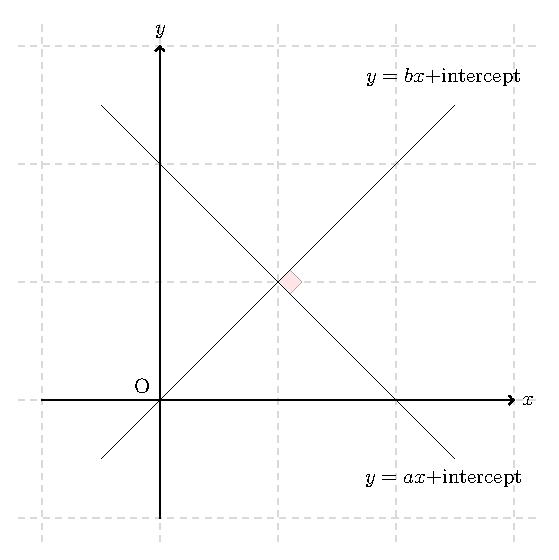
\includegraphics[width=0.6\textwidth]
{coordinates-and-slopes-1}
\caption{\textbf{Two Orthogonal Lines in a Cartesian Coordinate System}. 
\label{fig:slopes:01}}
\end{minipage}
\end{figure}

We have very little information to go by. Can we infer the slope $b$ from $a$? Consider a special case. Take the $45^{\circ}$ line and consider the line orthogonal to it that goes through the origin. The orthogonal line is clearly the $-45^{\circ}$ line --- or equivalently the $315^{\circ}$ line ($360-45$). In radians, the $45^{\circ}$ line has angle $\frac{\pi}{4}$, while the $-45^{\circ}$ line has angle $\frac{-\pi}{4}=\frac{7\pi}{8}\bmod2\pi$. By inspection and considerations of symmetry, the slope of the $-45^{\circ}$ line is clearly $-1$. So is the answer simply $b=-a$? No! Read on.

\begin{figure}[hpbt]
\begin{minipage}[b]{\textwidth}
\centering
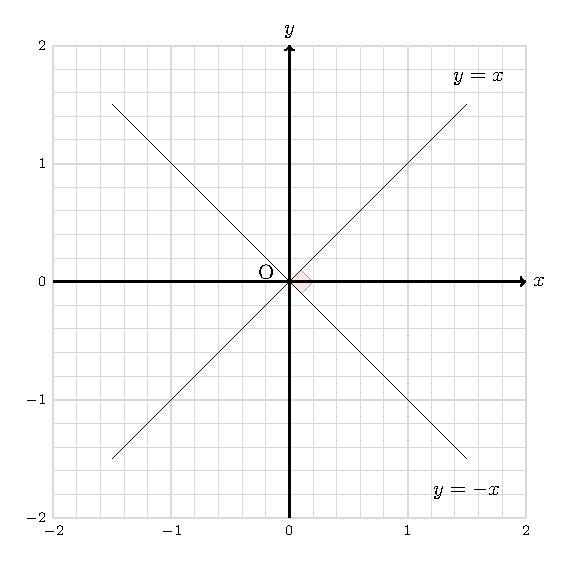
\includegraphics[width=0.6\textwidth]
{coordinates-and-slopes-2}
\caption{\textbf{Simple Example: The $45^{\circ}$ line}. 
\label{fig:slopes:02}}
\end{minipage}
\end{figure}

Consider now the general case. Since only the slope matters in this problem, we can take two lines that intersect at the origin. Figure~\ref{fig:slopes:02} shows that we can also represent the slopes graphically. As we are now considering two lines that intersect at the origin, their equations are simply $y=ax$ and $y=bx$. And so for $x=1$, say, we have $y=a$ on line $OA$ and $y=b$ on line $OB$. Can we find an expression for $b$ in terms of $a$? Amazingly we can! Thanks to several right triangles and the Pythagoras theorem.

\bigskip

Triangle $AOB$ yields:
\begin{align*}
(b-a)^2 = OA^2 + OB^2
\end{align*}

Triangle $OaA$ yields:
\begin{align*}
OA^2 = 1^2 + a^2
\end{align*}

Triangle $ObB$ yields:
\begin{align*}
OB^2 = 1^2 + b^2
\end{align*}

\begin{figure}[hpbt]
\begin{minipage}[b]{\textwidth}
\centering
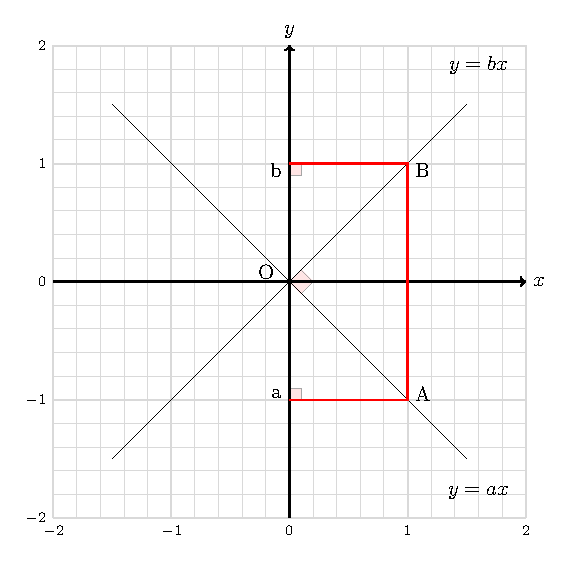
\includegraphics[width=0.6\textwidth]
{coordinates-and-slopes-3}
\caption{\textbf{Two Orthogonal Lines form Three Pythagorean Triangles}. 
\label{fig:slopes:02}}
\end{minipage}
\end{figure}

Putting it all together gives:
\begin{align*}
(b-a)^2 
  & = ~OA^2~~~ + ~~~OB^2 \\
  & = 1^2 + a^2 ~+~ 1^2 + b^2 \\
b^2 - 2ab + a^2 
  & = a^2 + b^2 + 2 \\
-2ab & = 2\\
ab & = -1
\end{align*}

The slope of any perpendicular line is therefore equal to \textbf{minus the inverse} slope:
\begin{alignbox*}
b = -\frac{1}{a}
\end{alignbox*}

\end{document}